%****************************************************************************
\documentclass[12pt]{article}
\usepackage{natbib}  % biliografia
\bibpunct{(}{)}{;}{a}{,}{,} % Apresentação bibliografia no texto
\usepackage[utf8]{inputenc}	 % Não necessidade de diferenciar caracteres especiais
\usepackage{graphicx, float} %% colocar figura no texto
\usepackage{amsmath,amsfonts,amssymb,amsthm} % Fórmulas
\usepackage[colorlinks=false, hidelinks]{hyperref}%% para fazer referência ao clicar
\usepackage{fancyhdr} % Controle de cabeçalho e rodapé
\usepackage[left=3cm,top=2.5cm,right=3cm,bottom=2.5cm,
headheight=1.25cm]{geometry} % Define margens
\usepackage{setspace} % Para espaçamento entre linhas

\setlength{\parindent}{0pt}

\pagestyle{fancy}
\fancyhf{}
% Cabeçalho
\fancyhead[RO]{ESAMP 2023}
% Rodapé
\fancyfoot[RO]{VI Escola de Amostragem e Métodos de Pesquisa}
\renewcommand{\footrulewidth}{0.4pt}

%****************************************************************************

\begin{document}

\onehalfspacing

\title{\Large\bf TÍTULO DO TRABALHO}
\author{%
	Autor 1${}^1$, \qquad Autor 2${}^1$, \qquad Autor 3${}^2$ \\[1.1ex]
    {\small email@autor1.com}\\
	\emph{\small ${}^1$ Filiação autores 1 e 2 - Cidade, País.} \\
        \emph{\small ${}^2$ Filiação autor 3 - Cidade, País.}
}
\date{}
\maketitle
\thispagestyle{fancy}

\section{Introdução}
Texto da Introdução.

Exemplo de citação \citep{bolfarine2005elementos}.

Exemplo de citação \cite{bolfarine2005elementos}

\section{Seção 2}
Texto da Seção 2.

\begin{figure}[htbp]
	\centering
 	% Título
        \caption{Figura Exemplo}
        % Define escala e seleciona imagem
		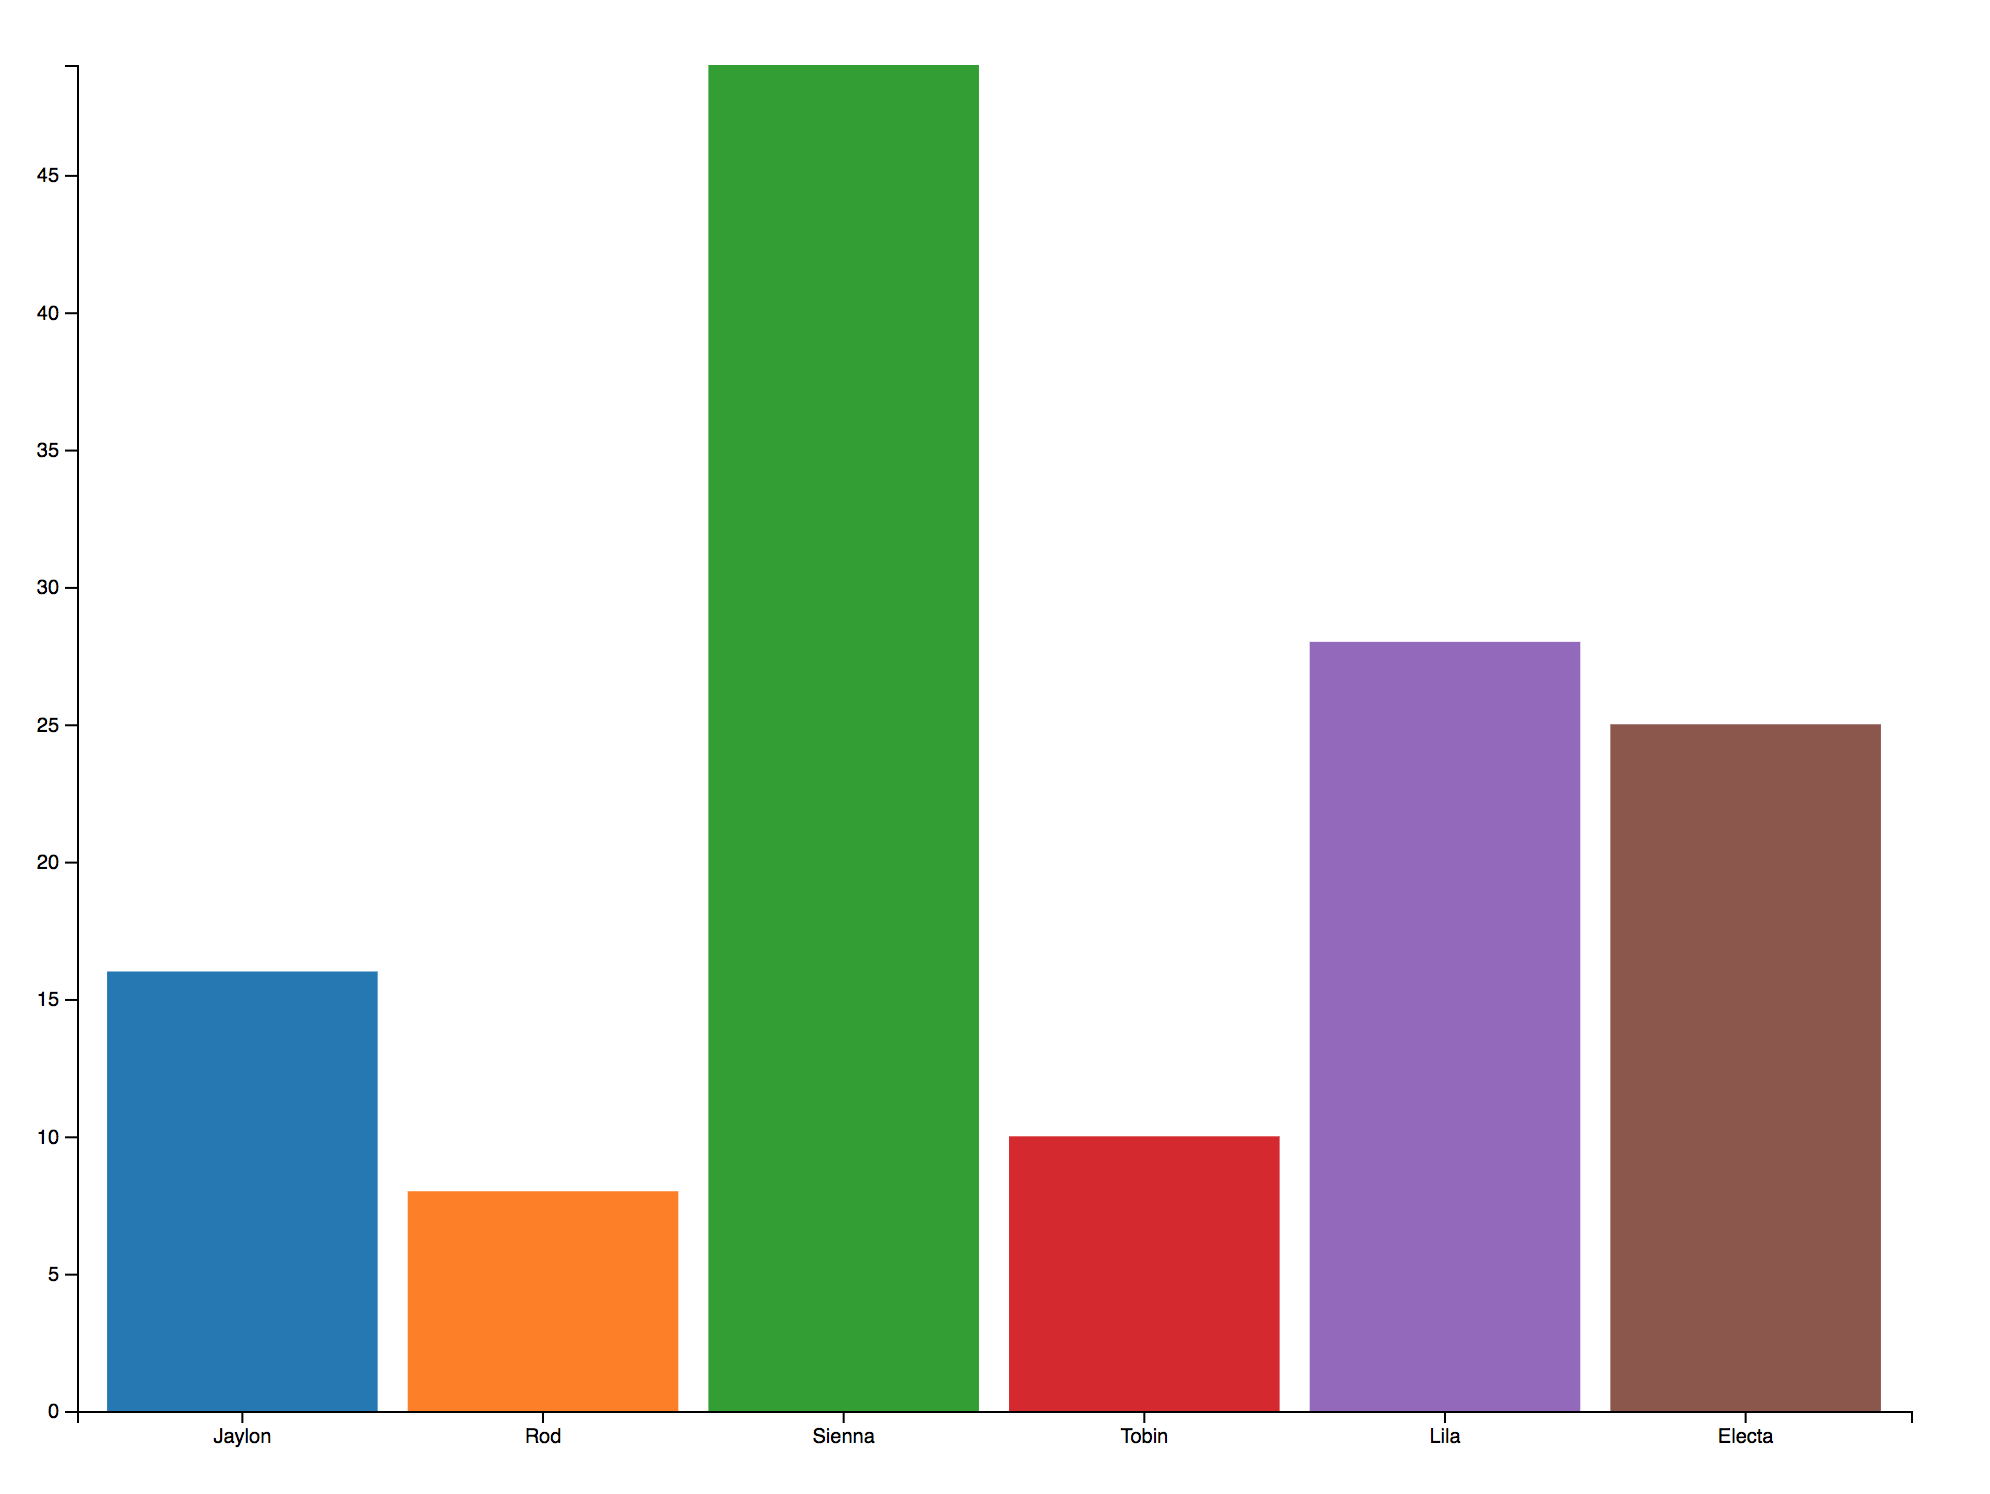
\includegraphics[scale=0.15]{exemplo_figura.png}
	% Rótulo para referenciar
        \label{rotulo_figura}\\
  \normalsize{Exemplo de \href{https://imgur.com/gallery/j8K7nfa}{Texto do hiperlink}.}
\end{figure}

Citando a figura \ref{rotulo_figura} no texto

\begin{table}[!htbp] \centering 
    % Título Tabela
    \caption{Tabela Exemplo} 
    % Rótulo para referenciar
    \label{rotulo_tabela} 
    \begin{tabular}{@{\extracolsep{5pt}} ccccc} 
        \\[-1.8ex]\hline 
        Col1 & Col2 & Col3 & Col4 \\ 
        \hline \\[-1.8ex] 
        Cat1 & 6  & 11 & 16 \\ 
        Cat2 & 7  & 12 & 17 \\ 
        Cat3 & 8  & 13 & 18 \\ 
        Cat4 & 9  & 14 & 19 \\ 
        Cat5 & 10 & 15 & 20 \\ 
        \hline \\[-1.8ex] 
        \small{Fonte: Teste}
    \end{tabular} 
\end{table} 

Referenciando Tabela \ref{rotulo_tabela}

\section{Conclusão}
Texto da Conclusão.


\section*{Agradecimentos}
Agradecimentos aos órgãos e agências de fomento à pesquisa, caso tenha.

\bibliography{referencias}
\bibliographystyle{apalike}

\end{document} 